\section{Data Analysis and Results}
In the following section, the hand-washing trials, the SRS survey, entrance survey, and post-interventions survey, and the parent interviews are analyzed qualitatively, and the annotated video data of the hand-washing trials is analyzed quantitatively.  

%need to comment what case selection is this, and its implications on our analysis and how to interpret the results
%sampling selection:
%which case is our participant?
%1. Key cases
%2. Outlier cases
%3. Local knowledge cases
%why this is good and why this is bad and what do we do now after knowing this?
\subsection{Participants Recruited}
Due to limitation of time, we were only able to recruit one subject.  Our participant is a thirteen years old male child (C) of Asian ethnicity.  He was accompanied to the trials by his mother (M), who was the one that answered all surveys.

\subsubsection{Entrance and SRS Survey Results}
The following backgrounds of C are reported by the entrance and SRS surveys.  The purpose of this section is to familiarize the reader with our participant and understand better the context that our study results situate in.

\paragraph{Child's Demographics and Inclusion Criteria Fit}
M reported that C has been clinically diagnosed of Autism Spectrum Disorder.  We also conducted the Social Responsiveness Scale Survey, and C obtained a T-score of 79, passing the minimum score for severe ASD.  Through the Entrance Survey, we learned that C has difficulty independently completing self-care activities (a 2 on a scale of 1 (not independent at all) to 5 (completely independent)), and this includes hand-washing (also a 2 on the same scale).  We also learned that C is able to do but not good at verbal communication (a 3 on a scale of 1 (very not well) to 5 (very well)).  Specifically, C can only speak one or two words at a time to express what he wants, uses iPad for communication, and often just murmurs illegibly.  However, C has the ability to follow simple, one-step verbal instructions (a 4 on a scale of 1 (very not well) to 5 (very well)).  Lastly, C does not exhibit severely aggressive behavior (a 1 from a scale of 1 (never) to 5 (often)).  The above shows that C fits in our inclusion criteria.

\paragraph{Child's Experience with Technologies}
C is more of a visual learner.  He uses a computer at home, and likes to use it very much.  He also likes to use other technologies (e.g. iPhone, iPad), and likes to watch movies and TV.  He doesn't have a robot toy to play with at home or at school, so M doesn't know how much he likes to play with robot toys.  The parent never used technologies to help C with self-care activities except using pictures to teach step by step hand-washing.

\paragraph{Child's Personal Preferences}
The child is sensitive to sound.  He likes Disney cartoon musics, and likes to watch his favorite cartoon scenes repeatedly on the iPad.  To reward C after a good behavior, M suggested the following rewards: give extra time to play on iPad, give him praises (e.g. good job), give children books to read and animal dinosaurs to play with, give M's iPhone since C's favorite musics are on there.

\paragraph{Child's Abilities on Hand-washing and on Other ADLs}
The parent agrees that C usually gets distracted when performing hand-washing.  To assist him, M mainly reminds him to put soap, rinse properly, and dry properly with towel.  He needs more prompting in these areas since he always washes in a hurry.

Other activities C needs help with include:  tooth brushing -- 2 hours/week; bathing -- 4.5 hours/week; dressing -- usually just hand the clothes to him, he knows how to put them on, but needs reminders of the order of the clothing, 7 hours/week.

\paragraph{Parent's Expectation and Concerns}
The parent expected the robot to be helpful in reminding C to put soap, rinse and dry more, similar to the role of M.  Some concerns M has include: C may be wondering why does he need to wash hands so many times repeatedly; C performs well in his comfort zone with the same environment, so it takes a while for C to get used to the lab environment.

%this is the qualitative data method section
\subsection{Qualitative Data Analysis Method}
%Qualitative analysis method:
%the constant comparative method (see Chapter
%Eight ). Tell us what this is and cite a couple of references. Tell us
%precisely how you plan to go about doing it. What will you do first?
%Second? Next? That is, tell the reader your step - by - step plan for
%analyzing your data. This is where you might talk about coding
%your data.

%this is the qualitative data results section
\subsection{Description and Analysis of Trials, Surveys and Interviews}


\subsubsection{Post-Intervention Survey for Parent}
The post-intervention survey results are presented in Table \ref{tab:PostInterventionSurveyData}.  We see that M was happy with all aspects of the robot as a prompting agent, but did not see it to be as good as herself yet.  The suggestions M made regarding the robot and the experiment are reported in the discussion section.

\begin{table}[H]
	\centering
	\begin{tabular}{ | p{12cm} | l | }
		\hline
		\textbf{Survey Question}	&	\textbf{Parent's Answer}	\\	\hline	\hline		
		Hand-washing steps break down was appropriate	&	Strongly Agree	\\	\hline
		My child understood the verbal prompts	&	Agree	\\	\hline
		Robot's verbal prompts were appropriate	&	Strongly Agree	\\	\hline
		The prompt wordings were similar to mine	&	Strongly Agree	\\	\hline
		The prompt voice and tone were appropriate	&	Strongly Agree	\\	\hline
		The prompt wordings were easy to understand	&	Strongly Agree \\	\hline
		My child understood the gesture prompts	&	Strongly Agree	\\	\hline
		The gesture prompts were appropriate	&	Strongly Agree	\\	\hline
		The gesture prompts were easy to understand	&	Agree	\\	\hline
		The physical appearance of robot is aesthetically pleasing	&	Agree	\\	\hline
		The attention grabber gestures were appropriate	&	Strongly Agree	\\	\hline
		The verbal rewards were appropriate	&	Strongly Agree	\\	\hline
		The reward gestures were appropriate	&	Strongly Agree	\\	\hline
		The robot was effective in assisting my child through hand-washing	&	Strongly Agree	\\	\hline
		The robot motivated my child to wash hands	&	Strongly Agree	\\	\hline
		The robot was fun for my child to use	&	Strongly Agree	\\	\hline
		My child was confused by the robot	&	Disagree	\\	\hline
		I like the idea of a robot prompting my child	&	Strongly Agree	\\	\hline
		The robot is able to provide guidance as well as I can or better	&	Neither Agree or Disagree	\\	\hline
		I would want to own a robot like this one	&	Strongly Agree	\\	\hline
	\end{tabular}
	\caption{The Post-Intervention Survey Data}
	\label{tab:PostInterventionSurveyData}
\end{table}


%rename this section to simply report sample selection
%when should i discuss parent's decision on how to involve during phase C?  should have been in the qualitative results section
\subsection{Experiment Design Change}
We were not able to counterbalance the confounding effect of learning through randomly assigning participants to phase orders (A-B-C versus A-C-B), since we only recruited one participant.  Instead, we decided to control it by splitting the Phase B into two segments, one before Phase C and one after.  Thus, we conducted the study in the following phase order: A-B-C-B (i.e. parent alone phase - robot alone phase - robot parent phase - 2nd robot alone phase).  This way, we can compare first Phase B and second Phase B to see how much does learning in Phase C affect our results.  Also, first Phase B and second Phase B won't have sixteen trials each due to limitation of time.  Instead, we conducted these two phases only long enough to see a stable response, as is typically done in a single-subject research design \cite{ayres2009acquisition, bereznak2012video}.  As a result, we had 16 trials for Phase A, 8 trials for first Phase B, 21 trials for Phase C, and 5 trials for second Phase B.  Note that the intervention conditions of first Phase B and second Phase B are meant to be the same.


\subsection{Video Data Analysis and Results}
\label{sec:VideoDataAnalysisAndResults}

\subsubsection{Analysis Method}
The analyses employed here are visual analyses.  The analyses mainly compare the levels (eyeballing the mean) of measures in different phases.  In cases where the level of a measure changes dramatically within a phase, this trend with initial level and final level were noted.

\subsubsection{Prompt Effectiveness}
To reflect how effective our prompting system is, we show whether the system can reduce both the number of incomplete steps and the number of parent prompts.

\paragraph{Number of Incomplete Steps}
We assumed that parent prompts had a higher level of authority over the child than robot prompts, because the robot only delivered verbal prompts and gestures such as pointing and motion demonstrations, while the parent could deliver those as well as nudging, guiding the arm, and completely executing the step for the child if the verbal and gesture prompts did not work.  This means we can measure the effect of robot prompts by comparing number of complete steps without prompts vs. with robot prompts alone, and measure the effect of parent prompts by comparing number of complete steps with robot prompts alone vs. with robot and parent prompts.  Figure \ref{fig:TotalNumberOfCompleteSteps} shows a series of plots for the measure ``Total Number of Complete Steps'', differing in what steps counted as completed when plotting the figures, e.g. Plot \ref{fig:7TotalNumberofCompleteSteps-WithoutPrompts} (``Without Prompts'') counts only steps completed by child with no prompts from the robot or the parent.  The next Plot \ref{fig:6TotalNumberofCompleteSteps-WithRobotPrompts} (``With Robot Prompts Only''), allows steps prompted by the robot to also count towards completed steps, and Plot \ref{fig:4TotalNumberofCompleteSteps-WithRobotAndParentPrompts} (``With Robot and Parent Prompts'') counts every completed steps even if they were prompted by the parent or the robot.

The most important comparison is between Plot \ref{fig:7TotalNumberofCompleteSteps-WithoutPrompts} (``Without Prompts'') and Plot \ref{fig:6TotalNumberofCompleteSteps-WithRobotPrompts} (``With Robot Prompts Only''), demonstrating the effectiveness of the robot's presence.  We see that parent alone phase (Phase A) was unaffected since robot wasn't present, but introducing the robot in the rest of the phases show effectiveness: robot alone phase (first Phase B) from 2.5 to 3, robot parent phase (Phase C) from 2 to 3, and robot alone repeat phase (second Phase B) from 2.5 to 4.

Comparing Plot \ref{fig:6TotalNumberofCompleteSteps-WithRobotPrompts} (``With Robot Prompts Only'') against Plot \ref{fig:4TotalNumberofCompleteSteps-WithRobotAndParentPrompts} (``With Robot and Parent Prompts''), we see the effectiveness of parent prompts: parent alone phase moved from 3 to 6, robot alone phase from 3 to 3.5, robot parent phase from 3 to 5, robot alone repeat phase from 4 to 4.5.
\begin{figure}[h]
	\centering
	\begin{subfigure}[b]{0.49\textwidth}
		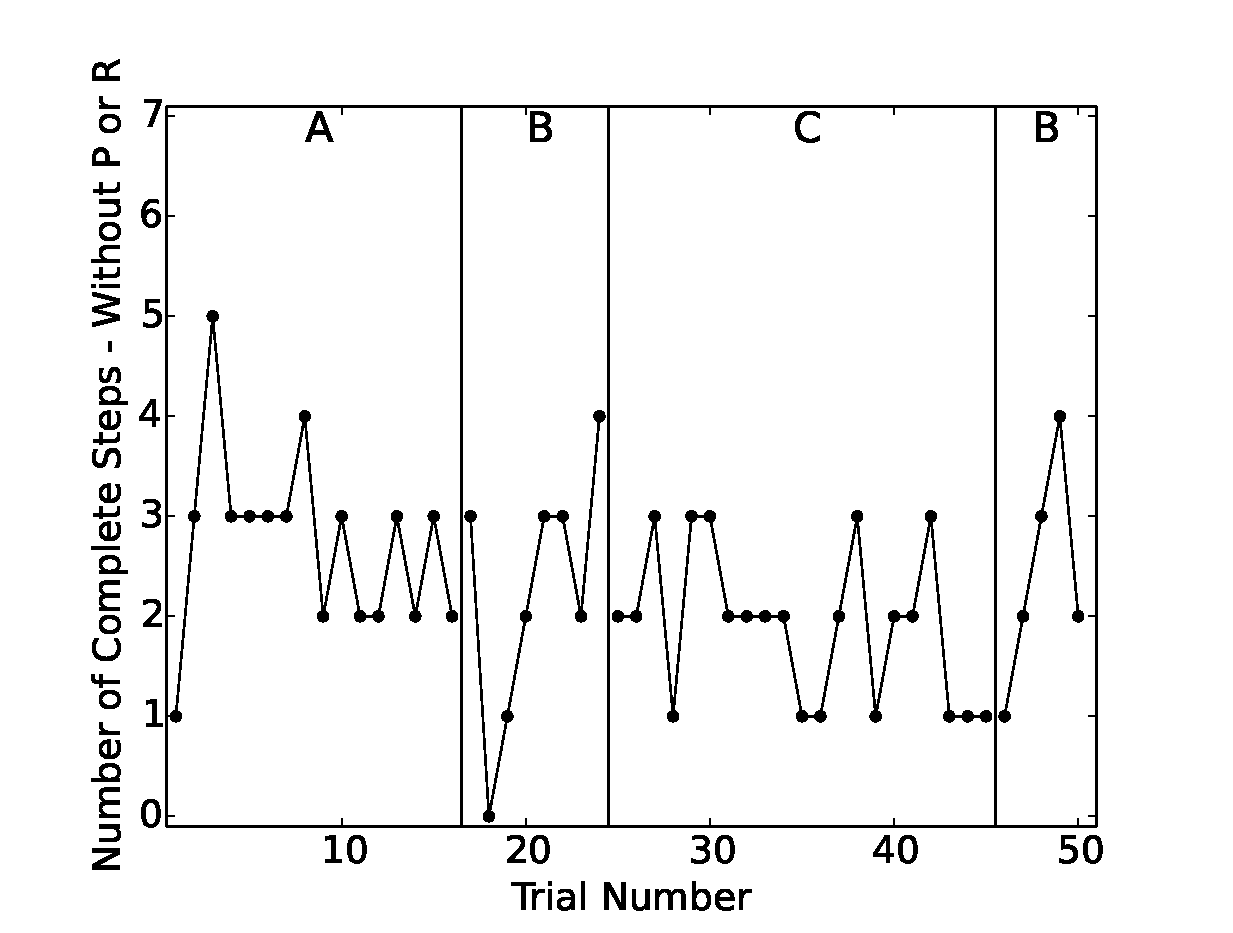
\includegraphics[width=1.1\linewidth]{./img/data_analysis/110NumberofCompleteSteps-WithoutPorR.eps}
		\caption{Total Number of Complete Steps - Without Prompts}
		\label{fig:7TotalNumberofCompleteSteps-WithoutPrompts}
	\end{subfigure}
	\hfill
	%	~ %add desired spacing between images, e. g. ~, \quad, \qquad, \hfill, or double enter etc.	
	\begin{subfigure}[b]{0.49\textwidth}
		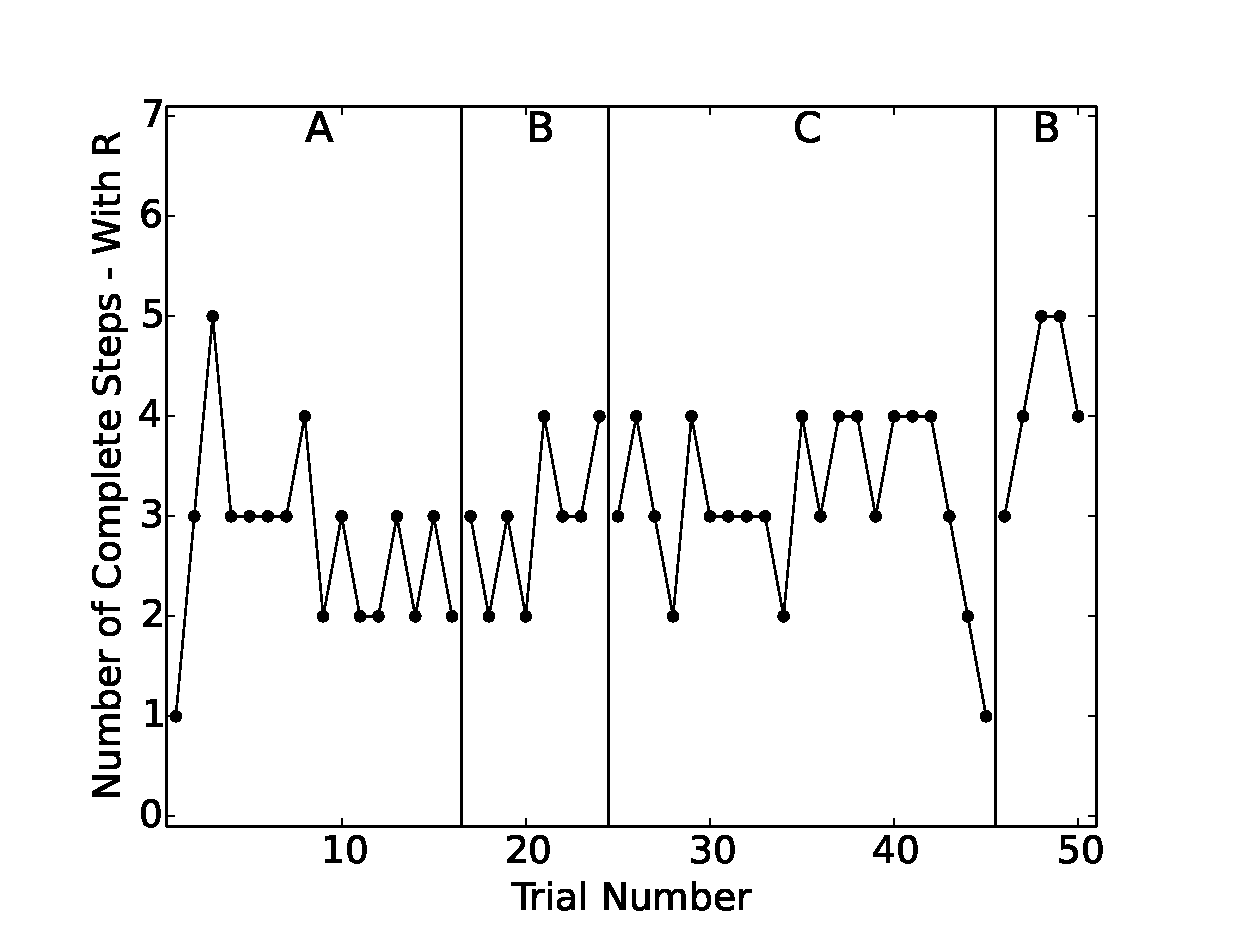
\includegraphics[width=1.1\linewidth]{./img/data_analysis/109NumberofCompleteSteps-WithR.eps}
		\caption{Total Number of Complete Steps - With Robot Prompts Only}
		\label{fig:6TotalNumberofCompleteSteps-WithRobotPrompts}
	\end{subfigure}%
	
	
	\begin{subfigure}[b]{0.49\textwidth}
		
\includegraphics[width=1.1\linewidth]{./img/data_analysis/blank.png}
	\end{subfigure}%
	\hfill
	\begin{subfigure}[b]{0.49\textwidth}
		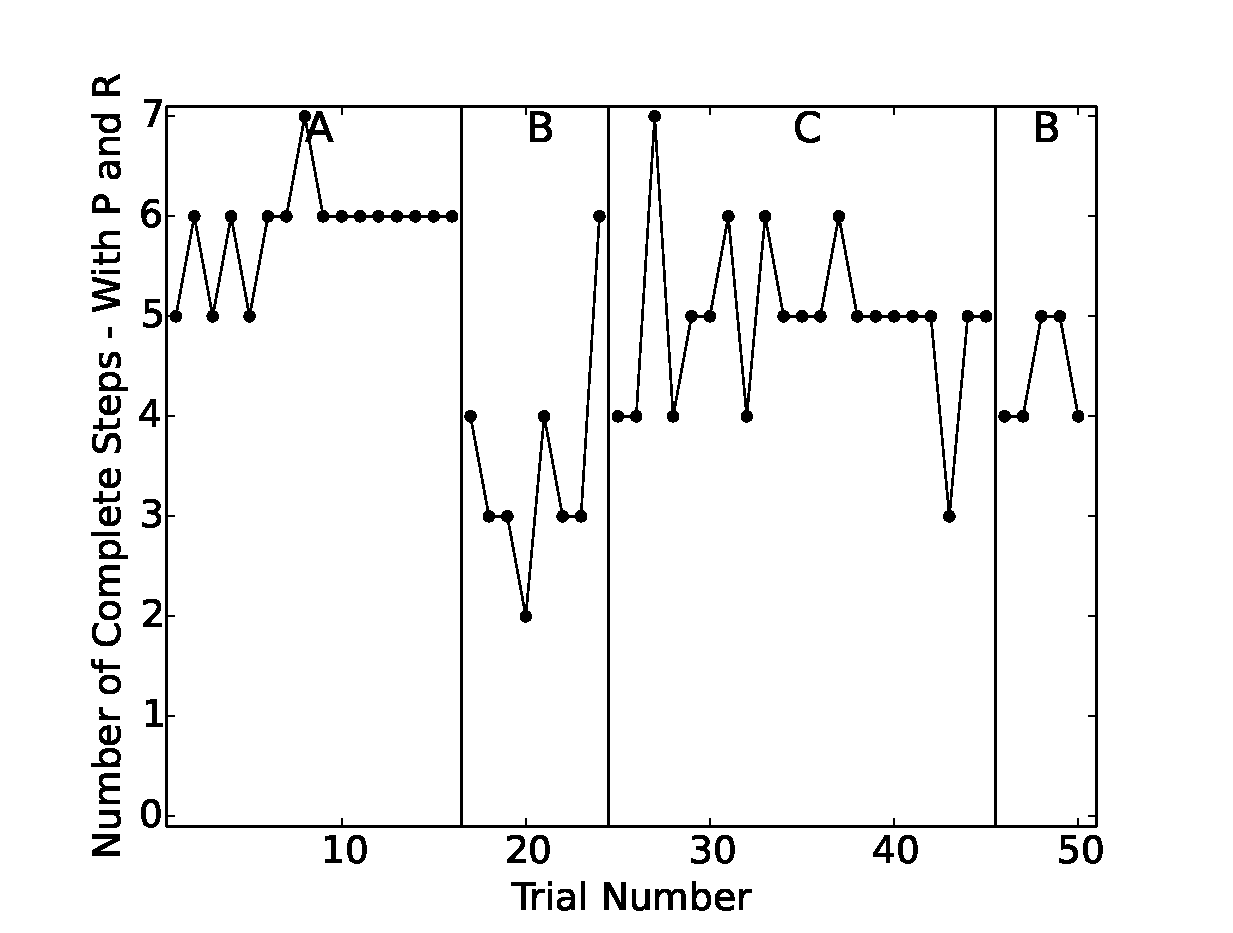
\includegraphics[width=1.1\linewidth]{./img/data_analysis/108NumberofCompleteSteps-WithPandR.eps}
		\caption{Total Number of Complete Steps - With Robot and Parent Prompts}
		\label{fig:4TotalNumberofCompleteSteps-WithRobotAndParentPrompts}
	\end{subfigure}%
	\caption{Total Number of Complete Steps}
	\label{fig:TotalNumberOfIncompleteSteps}
\end{figure}

\paragraph{Number of Parent Prompts}
The measure ``Total Number of Parent Prompts'' is plotted in Figure \ref{fig:TotalNumberOfParentPrompts}.  Plot \ref{fig:25TotalNumberofParentPrompts} is for the overall count (i.e. counting both physical and non-physical prompts).  It shows that during parent alone phase (A), the measure has an upward trend from 5 moving to 20.  However, in robot alone phase (first Phase B), we have a sudden drop leveling at near zero.  In robot parent phase (C), the measure has a downward trend moving from 15 to 5.  In robot alone repeat phase (second Phase B), we again observe a near zero level.  By comparing the measures across phases, we see that the robot's presence were effective in reducing the number of parent prompts, especially in robot alone and repeat phases.  Plot \ref{fig:26TotalNumberofParentPrompts-Physical} is for the physical prompt count.  This plot shows when the parent resorts to a higher prompt level (i.e. physical prompts such as nudging, guiding, and physically intervene) in order to get the child's compliance.  We see that the level is mainly near zero for all phases except for robot parent phase (C), leveling around 2.5.
\begin{figure}[h]
	\centering
	\begin{subfigure}[b]{0.49\textwidth}
		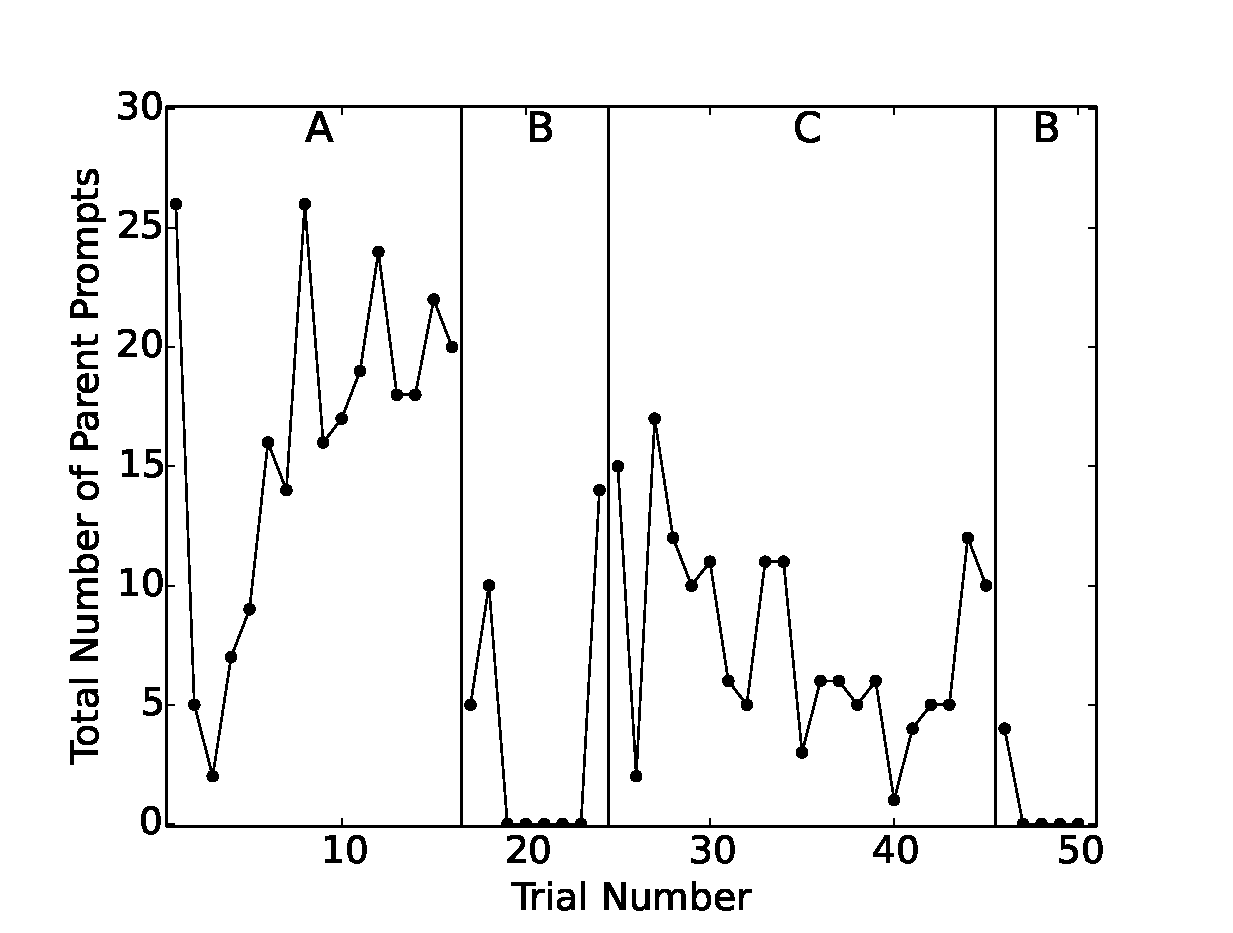
\includegraphics[width=1.1\linewidth]{./img/data_analysis/25TotalNumberofParentPrompts.eps}
		\caption{Total Number of Parent Prompts - Overall}
		\label{fig:25TotalNumberofParentPrompts}
	\end{subfigure}
	\hfill
	\begin{subfigure}[b]{0.49\textwidth}
		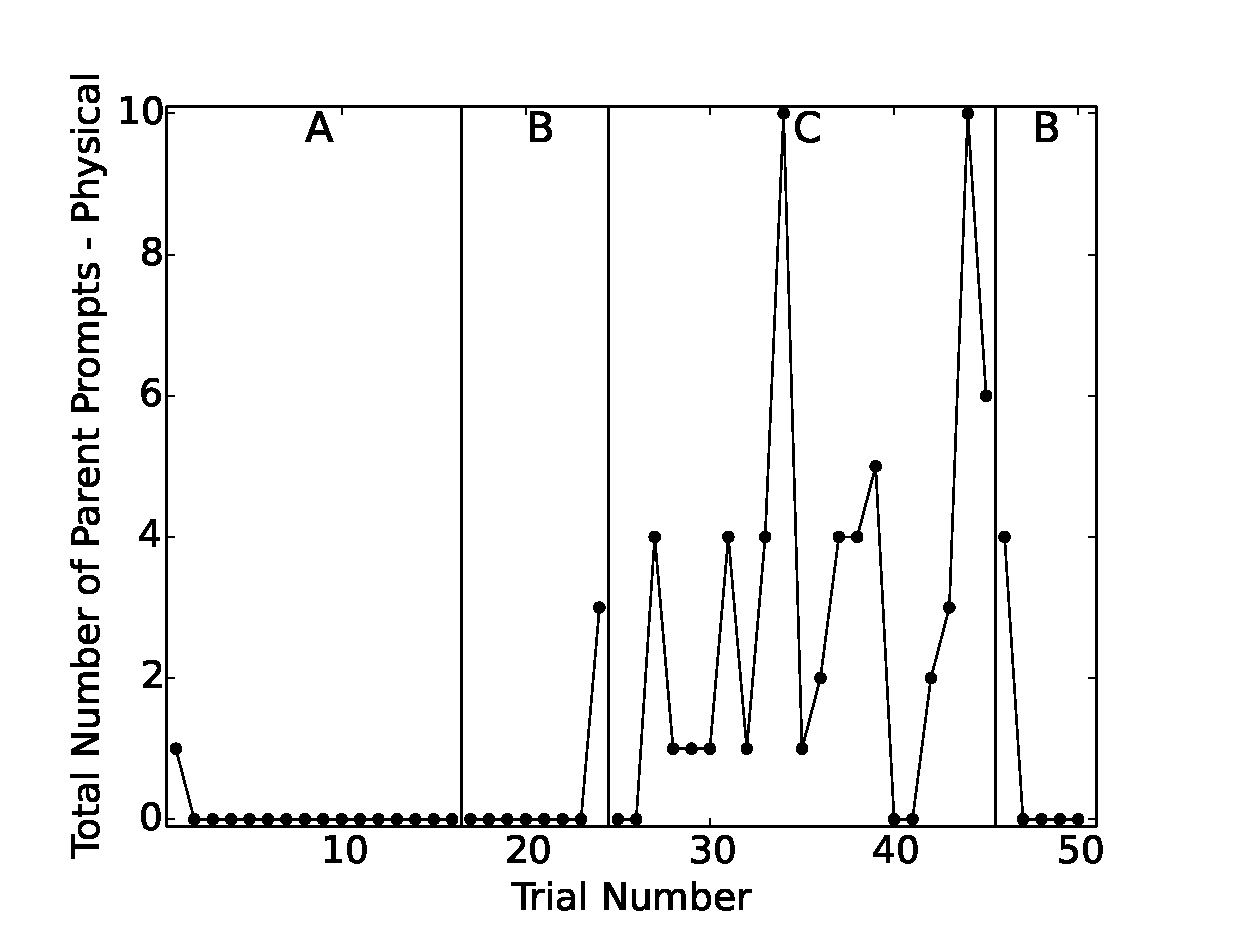
\includegraphics[width=1.1\linewidth]{./img/data_analysis/26TotalNumberofParentPrompts-Physical.eps}
		\caption{Total Number of Parent Prompts - Physical}
		\label{fig:26TotalNumberofParentPrompts-Physical}
	\end{subfigure}%
	\caption{Total Number of Parent Prompts}
	\label{fig:TotalNumberOfParentPrompts}
\end{figure}


\subsubsection{Child's Response to Prompts}
To illustrate the child's different responses to the prompts, we characterized child's responses into three categories: ``compliance'', ``not affected by prompt'', and others.

\paragraph{Compliance Rate}
A response is counted towards ``compliance'' if the child executes the correct step in response to the prompt.  If the child was executing the wrong step before prompt, and is converted into doing the correct step due to prompt, we call this hard compliance.  The compliance and hard compliance response rates are shown in Figure \ref{fig:ComplianceRate}.

Plot \ref{fig:102ComplianceRate-Overall} shows the overall compliance rate, with parent alone phase (A) leveling at 80\%, robot alone phase (first Phase B) leveling at 30\%, parent robot phase (C) moving upward from 60\% to 80\%, and robot alone repeat phase (second Phase B) leveling at 80\%.  We see that when the robot was first introduced in robot alone phase (first Phase B), the child did not comply to the prompts.  However, by going through Phase C where the parent prompts for child to follow the robot, the child complies more readily in the robot alone repeat phase, achieving similar level of compliance as the parent alone phase.  We need to note that this plot includes prompts delivered by the robot, by the parent, and by them together.  Even in robot alone and repeat phases, the parent still comes into the washroom and prompts when the child isn't complying to the robot.  To see whether the robot alone can potentially guide the child through the whole hand-washing activity with minimal parent involvement, we plotted the compliance rate counted over only prompts delivered by the robot, shown in Plot \ref{fig:79ComplianceRate-R1Pv0g0}.  This plot confirms the levels observed in the overall plot, validating the improvement of compliance rate seen in R Alone Rep phase.  To investigate to what extent the child is compliant, the overall hard compliance rate is shown in Plot \ref{fig:103HardComplianceRate-Overall}, with parent alone phase (A) split leveling at 100\% and 35\%, robot alone phase (first Phase B) leveling at 25\%.  The robot parent phase (C) averaging around 60\% but the spread increases as trials went on.  Lastly, the robot alone repeat phase (second Phase B) levels at 50\%.  Similar to above, we observe an improvement of hard compliance between robot alone and repeat phases.  Looking at the robot prompts only Plot \ref{fig:92HardComplianceRate-R1Pv0g0}, the robot alone phase (first Phase B) drops to almost 0\%, while robot alone repeat phase (second Phase B) remains at 50\%.
\begin{figure}[h]
	\centering
	\begin{subfigure}[b]{0.49\textwidth}
		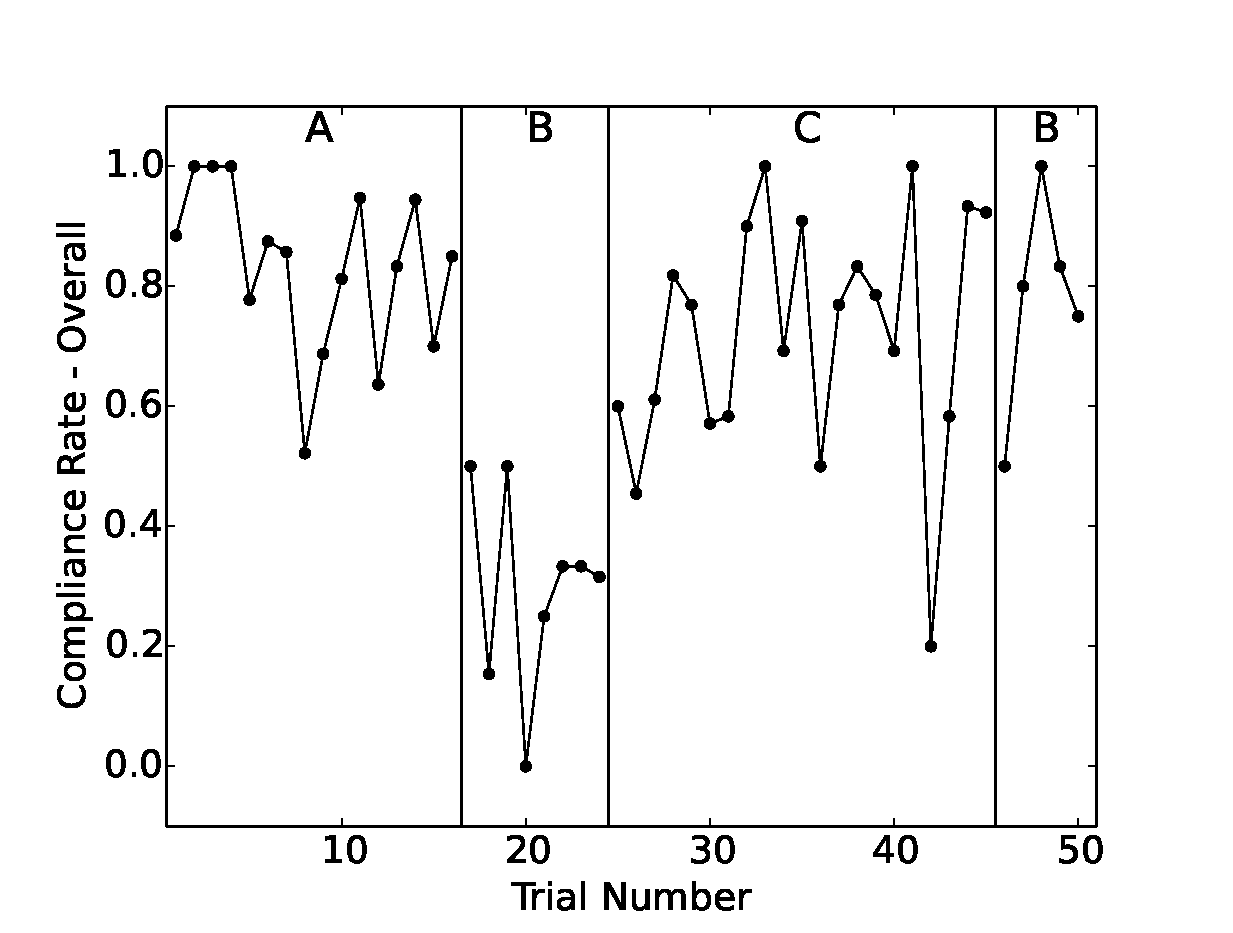
\includegraphics[width=1.1\linewidth]{./img/data_analysis/102ComplianceRate-Overall.eps}
		\caption{Compliance Rate - Overall}
		\label{fig:102ComplianceRate-Overall}
	\end{subfigure}
	\hfill
	\begin{subfigure}[b]{0.49\textwidth}
		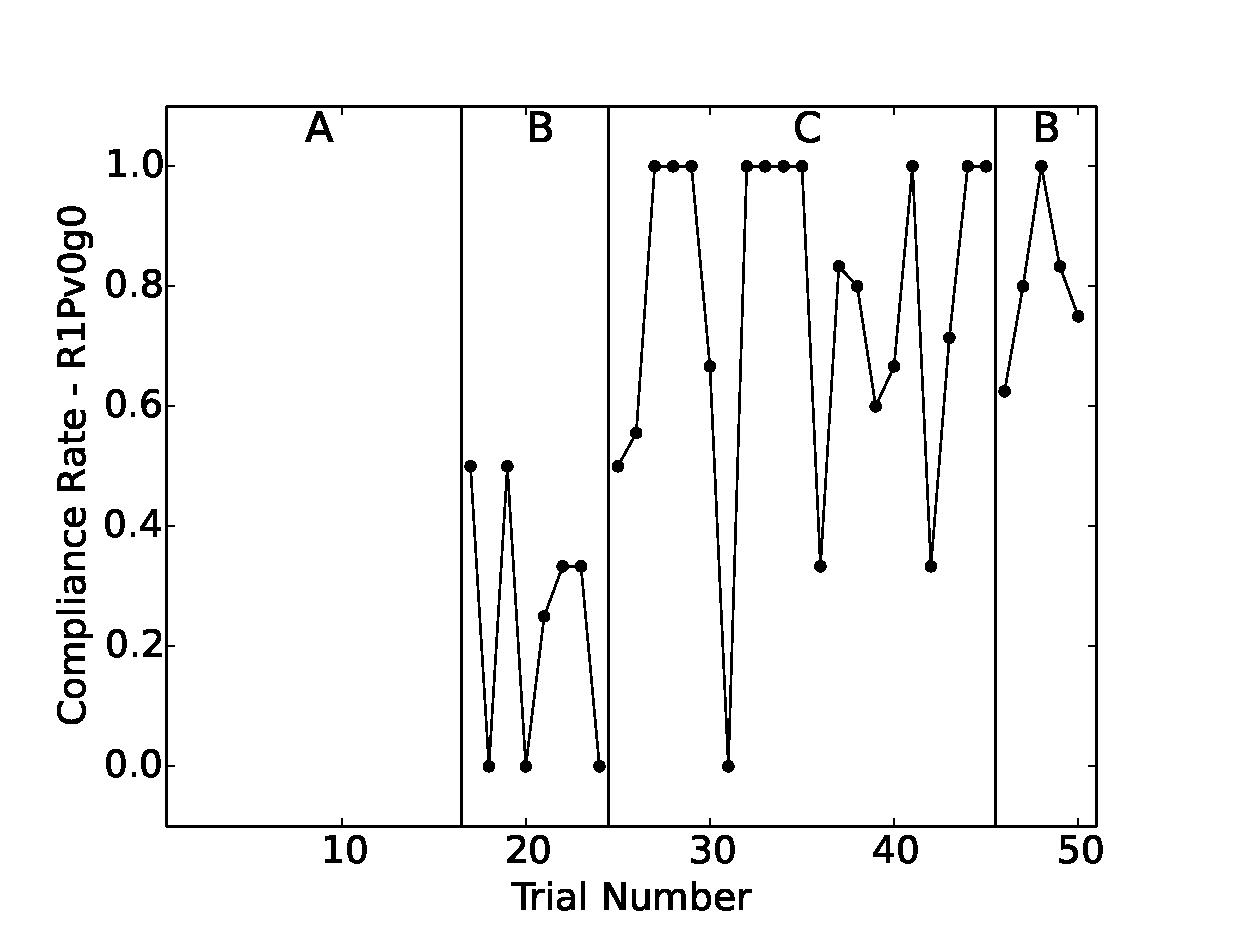
\includegraphics[width=1.1\linewidth]{./img/data_analysis/79ComplianceRate-R1Pv0g0.eps}
		\caption{Compliance Rate - Robot Only Prompts}
		\label{fig:79ComplianceRate-R1Pv0g0}
	\end{subfigure}%
	
	
	\begin{subfigure}[b]{0.49\textwidth}
		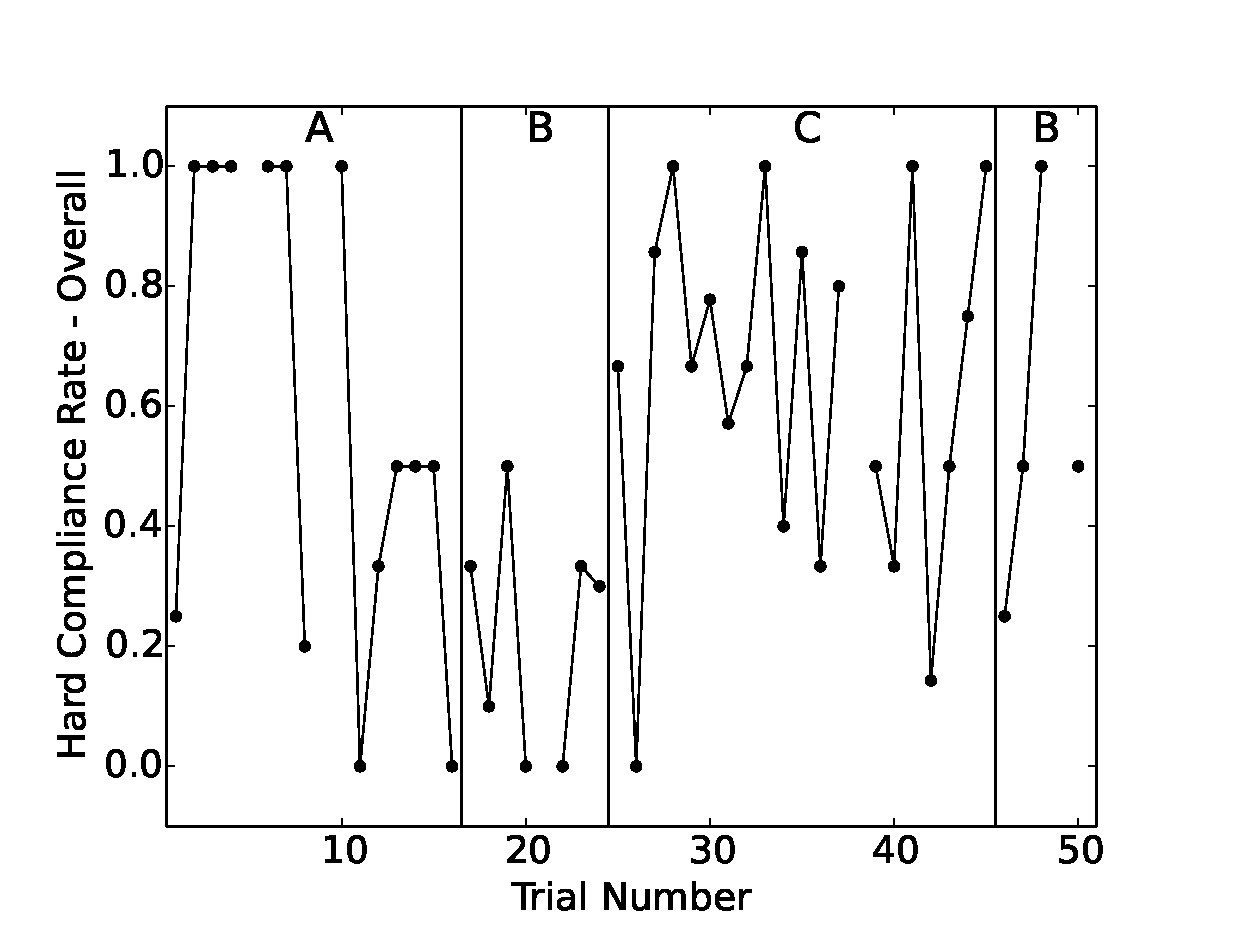
\includegraphics[width=1.1\linewidth]{./img/data_analysis/103HardComplianceRate-Overall.eps}
		\caption{Hard Compliance Rate - Overall}
		\label{fig:103HardComplianceRate-Overall}
	\end{subfigure}
	\hfill
	\begin{subfigure}[b]{0.49\textwidth}
		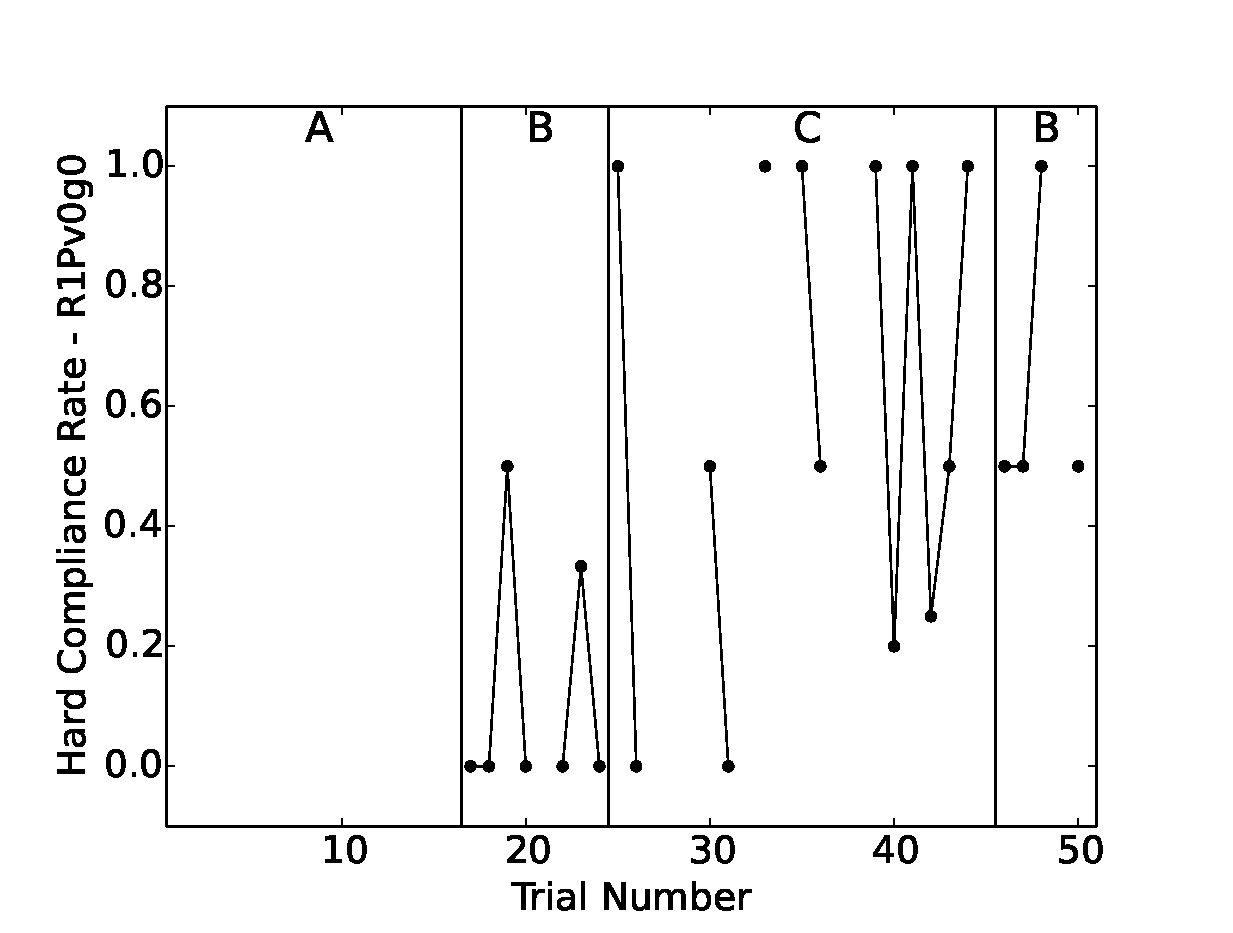
\includegraphics[width=1.1\linewidth]{./img/data_analysis/92HardComplianceRate-R1Pv0g0.eps}
		\caption{Hard Compliance Rate - Robot Only Prompts}
		\label{fig:92HardComplianceRate-R1Pv0g0}
	\end{subfigure}%
	\caption{Compliance Rate}
	\label{fig:ComplianceRate}
\end{figure}

\paragraph{Not Affected By Prompt Rate}
A response is counted towards ``not affected by prompt'' if the child was executing a wrong step and did not change after the prompt or was idling and did not change after the prompt.  The not affected by prompt rate is shown in Plot \ \ref{fig:99NotAffectedByPromptRate-Overall}.  We see that for most phases, it levels at 15\%, but for robot alone repeat phase (second Phase B) it is at 35\%.  This shows the robot prompts were ignored more when the robot was first introduced, but improves to an acceptable level through Phase C.
\begin{figure} [h]
	\centering
	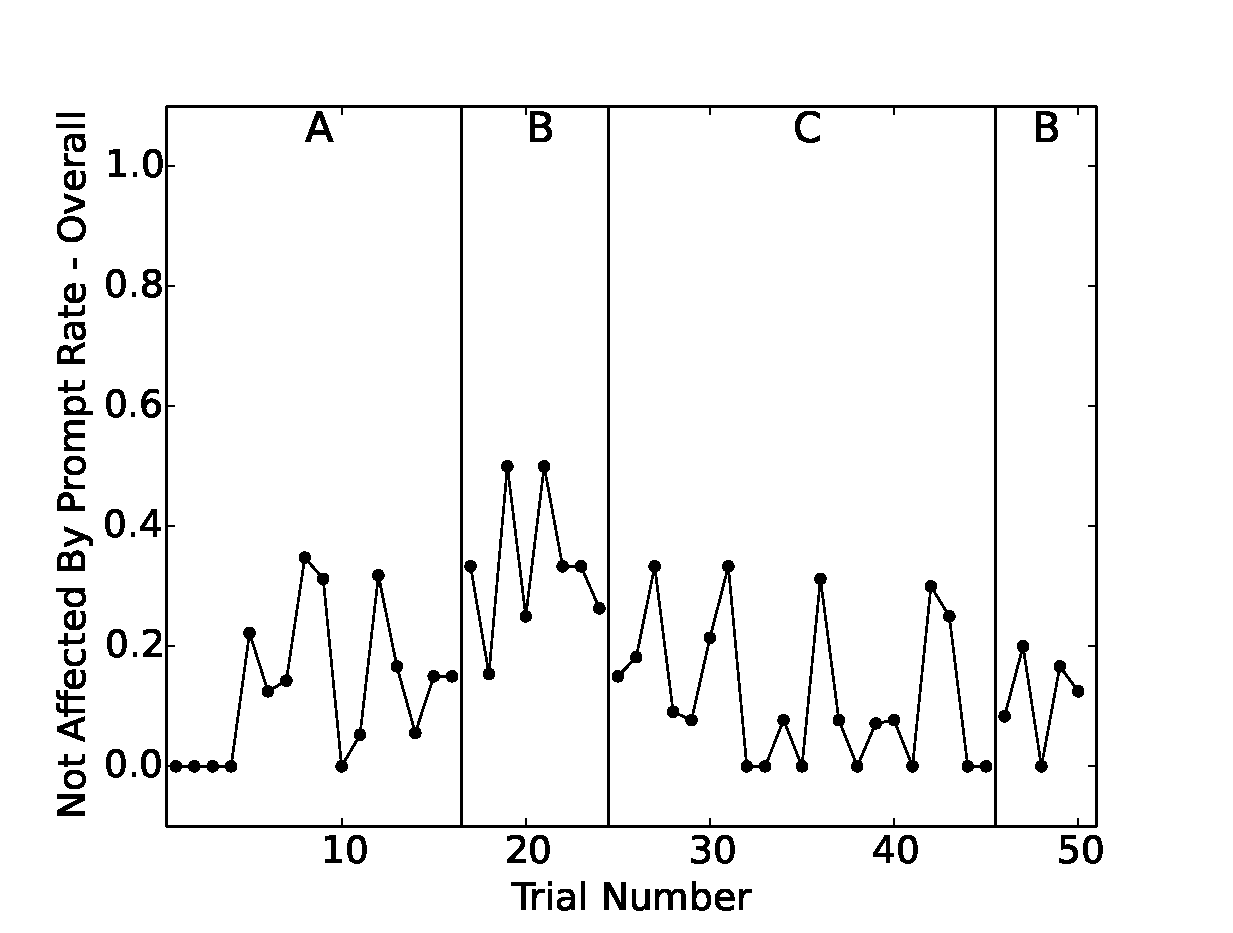
\includegraphics[width=0.6\textwidth]{./img/data_analysis/99NotAffectedByPromptRate-Overall.eps}
	\caption{Not Affected By Prompt Rate}
	\label{fig:99NotAffectedByPromptRate-Overall}
\end{figure}


\subsubsection{Engagement and Visual Attention}
To further characterize child's response to different prompting phases, we investigate how many times the child smiles and murmurs during step execution, and how often the child looks at the prompting agent during prompting and step execution.

\paragraph{Number of Times Child Smiles}
The measure "Total Number of Times Child Smiles" is shown in Plot \ \ref{fig:12TotalNumberofTimesChildSmiles}.  In it, parent alone phase (A) levels at 1.5, robot alone phase (first Phase B) levels at 0.5, robot parent phase (C) has a large spread and averages around 3, and robot alone repeat phase (second Phase B) also has a large spread and averages around 4.  It shows that the child smiles much more in later phases compared to earlier phases, and particularly, smiles in the repeat phase more than in robot alone phase.
\begin{figure} [h]
	\centering
	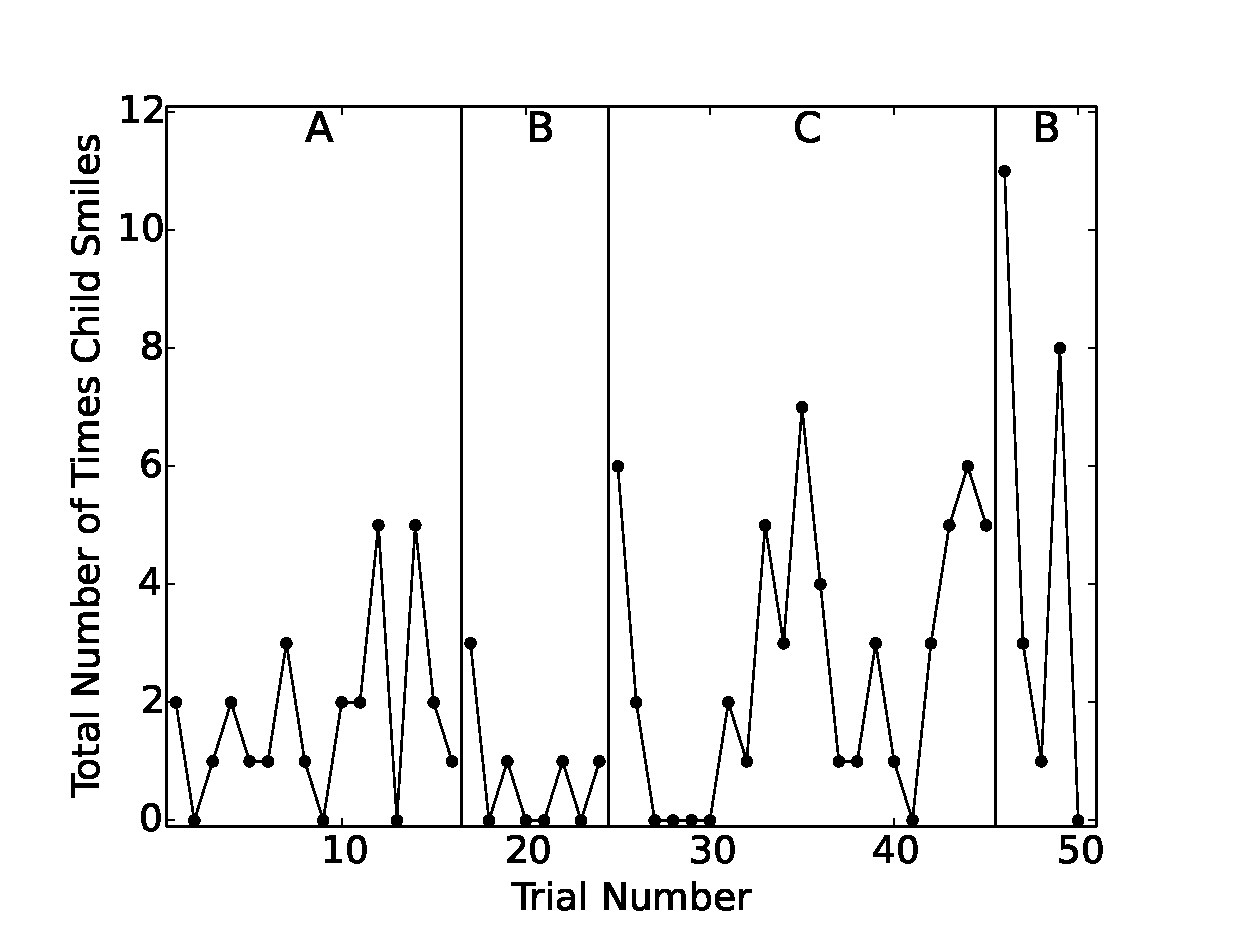
\includegraphics[width=0.6\textwidth]{./img/data_analysis/12TotalNumberofTimesChildSmiles.eps}
	\caption{Total Number of Times Child Smiles}
	\label{fig:12TotalNumberofTimesChildSmiles}
\end{figure}



\paragraph{Number of Times Child Murmurs}
The measure "Total Number of Times Child Murmurs" is shown in Plot \ \ref{fig:13TotalNumberofTimesChildMurmurs}.  In it, parent alone phase (A) has a large spread, averaging around 4.  Robot alone phase (first Phase B) levels at 0.5.  Robot parent phase (C) has a large spread, averaging around 4.  Robot alone repeat phase (second Phase B) levels at 2.  It shows that the child murmurs much more often when the parent is present.  Also, child murmurs in the repeat phase more than the robot alone phase.
\begin{figure} [h]
	\centering
	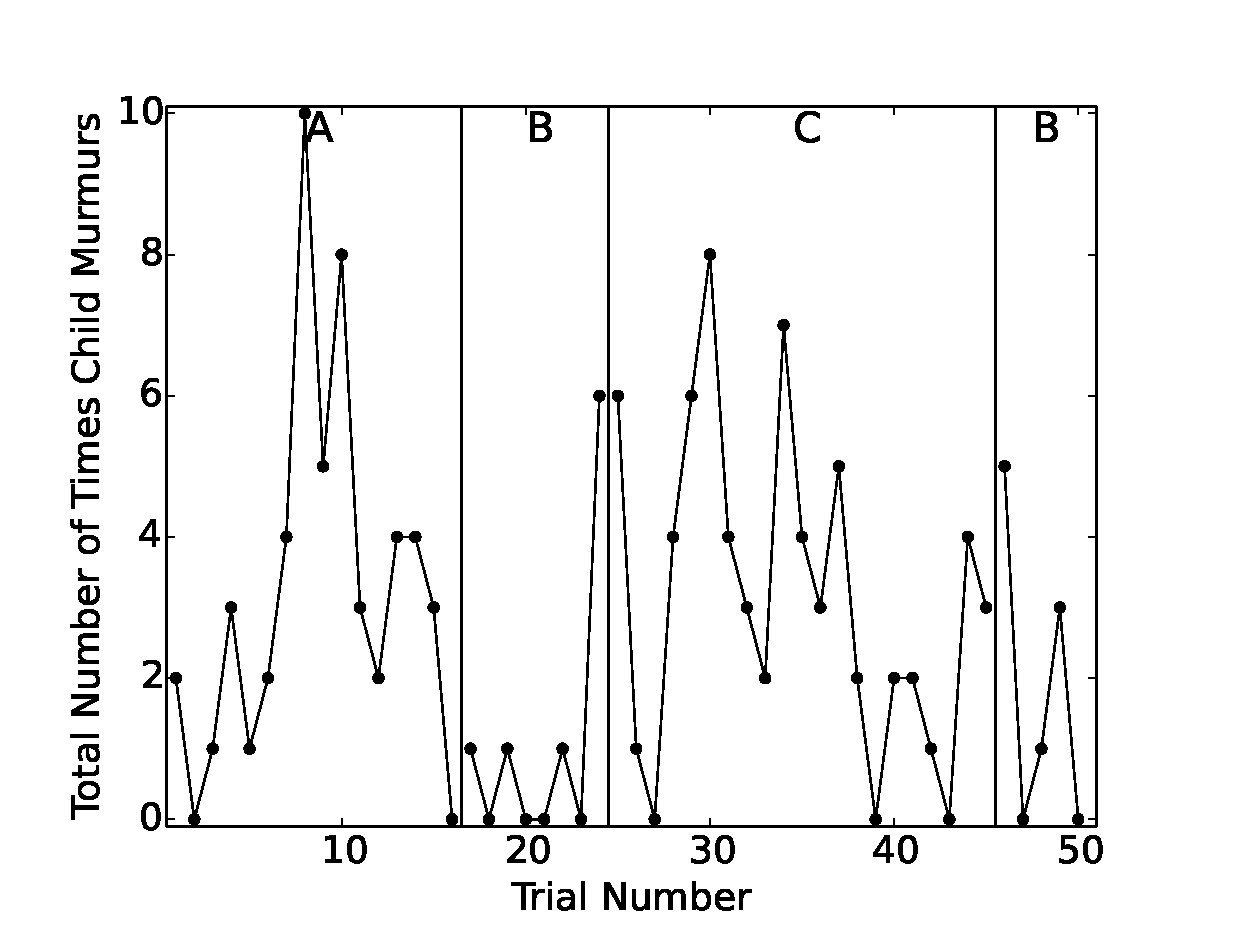
\includegraphics[width=0.6\textwidth]{./img/data_analysis/13TotalNumberofTimesChildMurmurs.eps}
	\caption{Total Number of Times Child Murmurs}
	\label{fig:13TotalNumberofTimesChildMurmurs}
\end{figure}

\paragraph{Looking at Prompting Agent Rate}
A prompt can be given by the parent, by the robot, or by them together.  During prompting and during step execution, the child may turn and look at the parent and/or the robot.  The gaze behavior of the child is shown in Figure \ref{fig:LookingAtPromptingAgentDuringPrompts} for all the cases above.  Because not all cases have the same amount of data in all phases, we will only mention here the phases that have enough evidence.  In Plot \ref{fig:8LookingatParentRateGivenParentPrompted}, ``Looking at Parent Rate - Given Parent Prompted'' levels at 40\% in parent alone phase (A).  In Plot \ref{fig:92HardComplianceRate-R1Pv0g0}, ``Looking at Robot Rate - Given Robot Prompted'' trends downward from 50\% to 30\% for robot alone phase (first Phase B), levels at 30\% with high spread for robot parent phase (C), and levels at 20\% for robot alone repeat phase (second Phase B).  We see that when the parent and the robot prompt individually, the parent has a higher chance of getting the child's visual attention.  Although the robot had similar levels of attention when was first introduced, it dropped as the study went on.  In Plot \ref{fig:10LookingatParentRateGivenBothPrompted}, ``Looking at Parent Rate - Given Both Prompted'' averages around 50\% with high spread in robot parent phase (C).  In Plot \ref{fig:11LookingatRobotRateGivenBothPrompted}, ``Looking at Robot Rate - Given Both Prompted' levels at 15\% for robot parent phase (C).  We see that when the parent and the robot prompt at the same time, the parent had a greater amount of visual attention.  It is interesting to note that the parent had similar levels of visual attention when prompting alone and when prompting with the robot.  The robot, however, experienced a decrease in visual attention level when the parent prompts with it.
\begin{figure}[h]
	\centering
	\begin{subfigure}[b]{0.49\textwidth}
		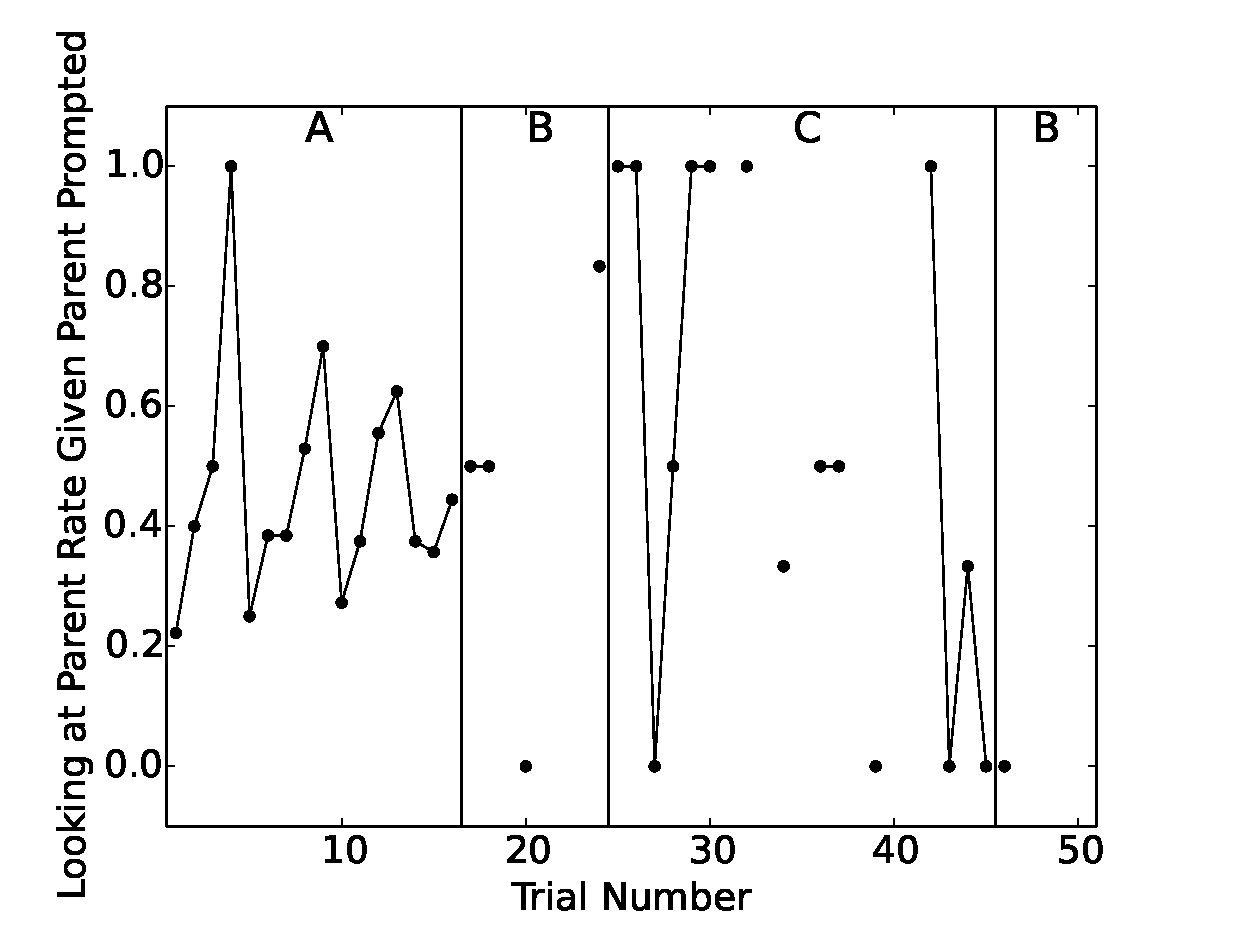
\includegraphics[width=1.1\linewidth]{./img/data_analysis/8LookingatParentRateGivenParentPrompted.eps}
		\caption{Looking at Parent Rate - Given Parent Prompted}
		\label{fig:8LookingatParentRateGivenParentPrompted}
	\end{subfigure}
	\hfill
	\begin{subfigure}[b]{0.49\textwidth}
		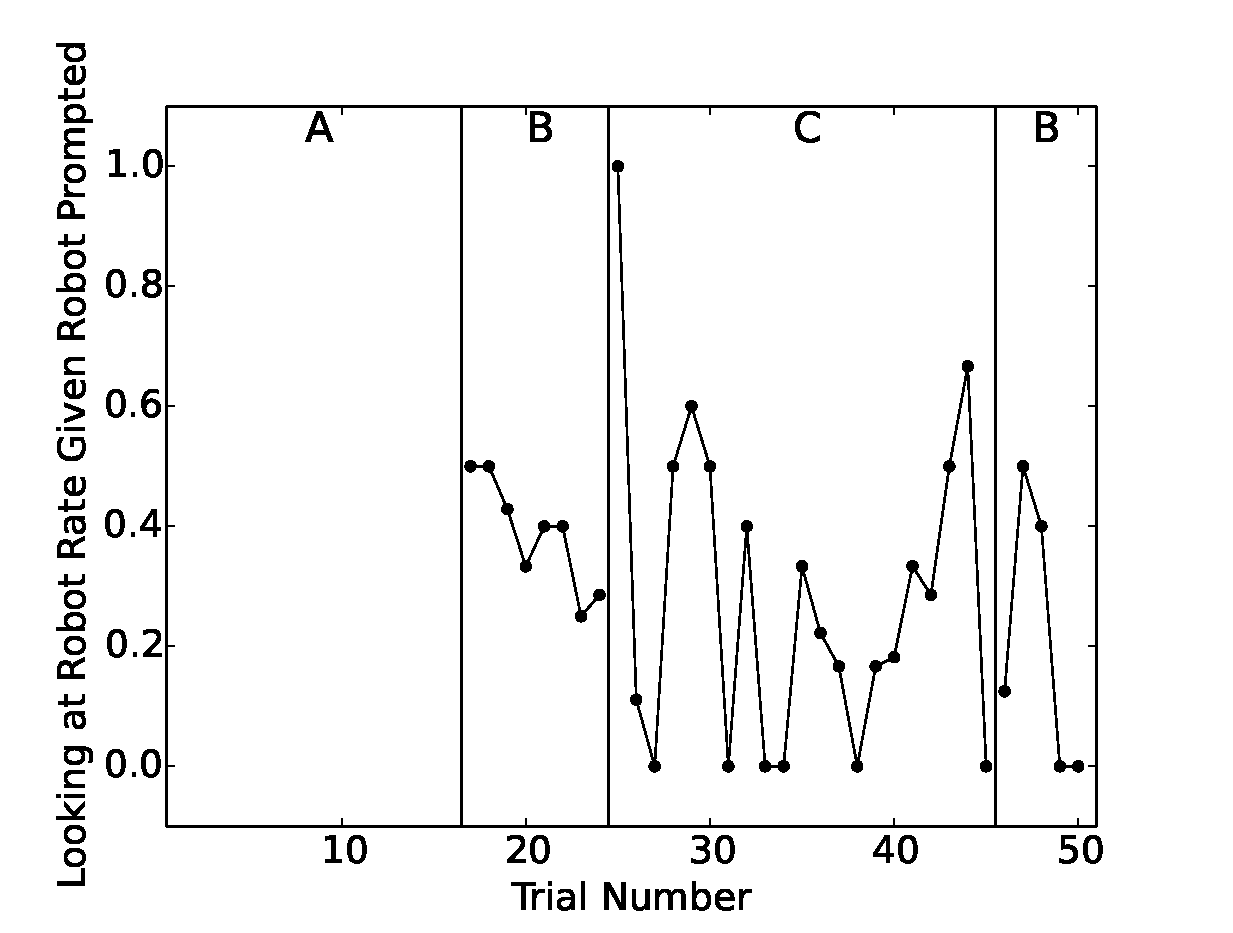
\includegraphics[width=1.1\linewidth]{./img/data_analysis/9LookingatRobotRateGivenRobotPrompted.eps}
		\caption{Looking at Robot Rate - Given Robot Prompted}
		\label{fig:9LookingatRobotRateGivenRobotPrompted}
	\end{subfigure}%
	
	
	\begin{subfigure}[b]{0.49\textwidth}
		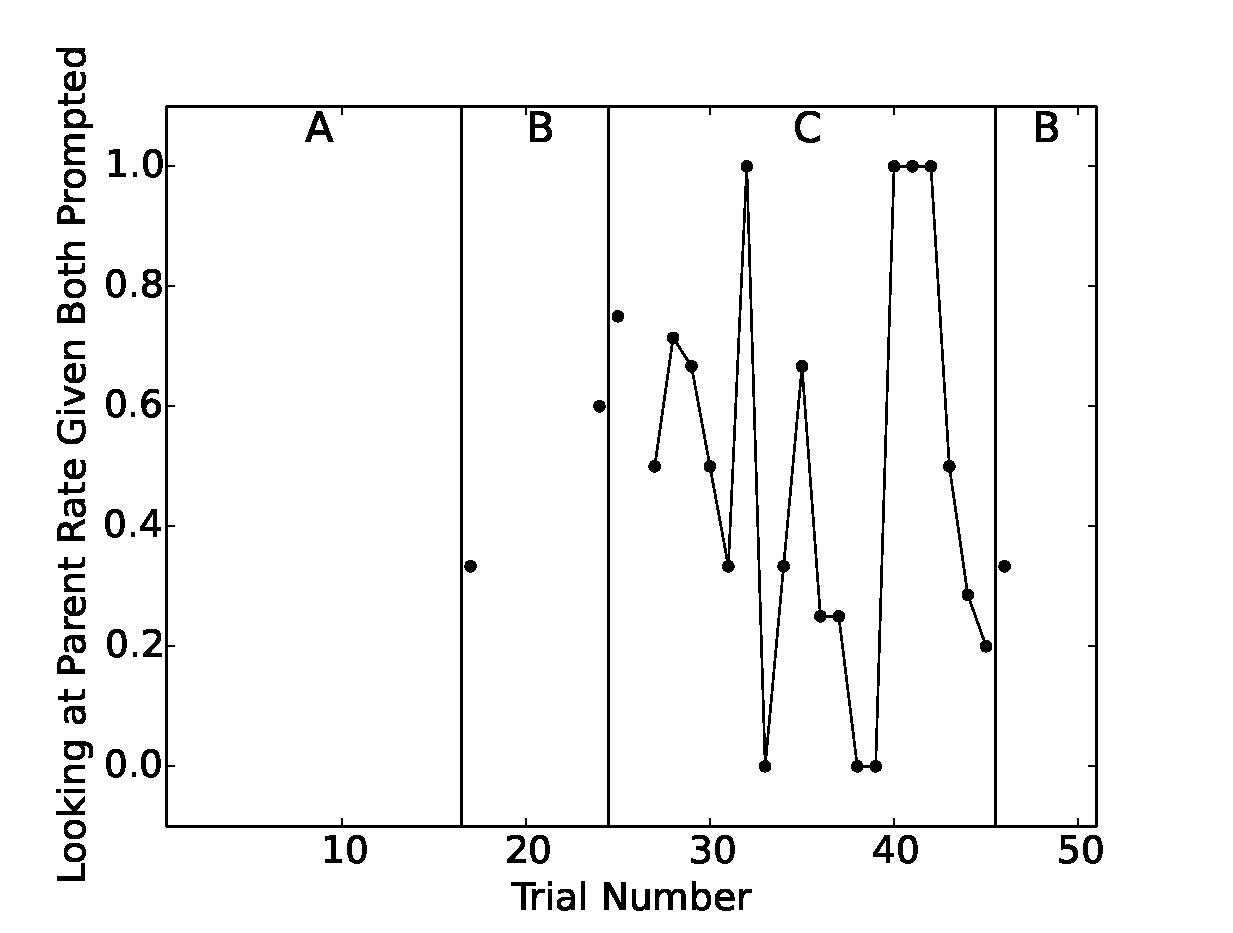
\includegraphics[width=1.1\linewidth]{./img/data_analysis/10LookingatParentRateGivenBothPrompted.eps}
		\caption{Looking at Parent Rate - Given Both Prompted}
		\label{fig:10LookingatParentRateGivenBothPrompted}
	\end{subfigure}
	\hfill
	\begin{subfigure}[b]{0.49\textwidth}
		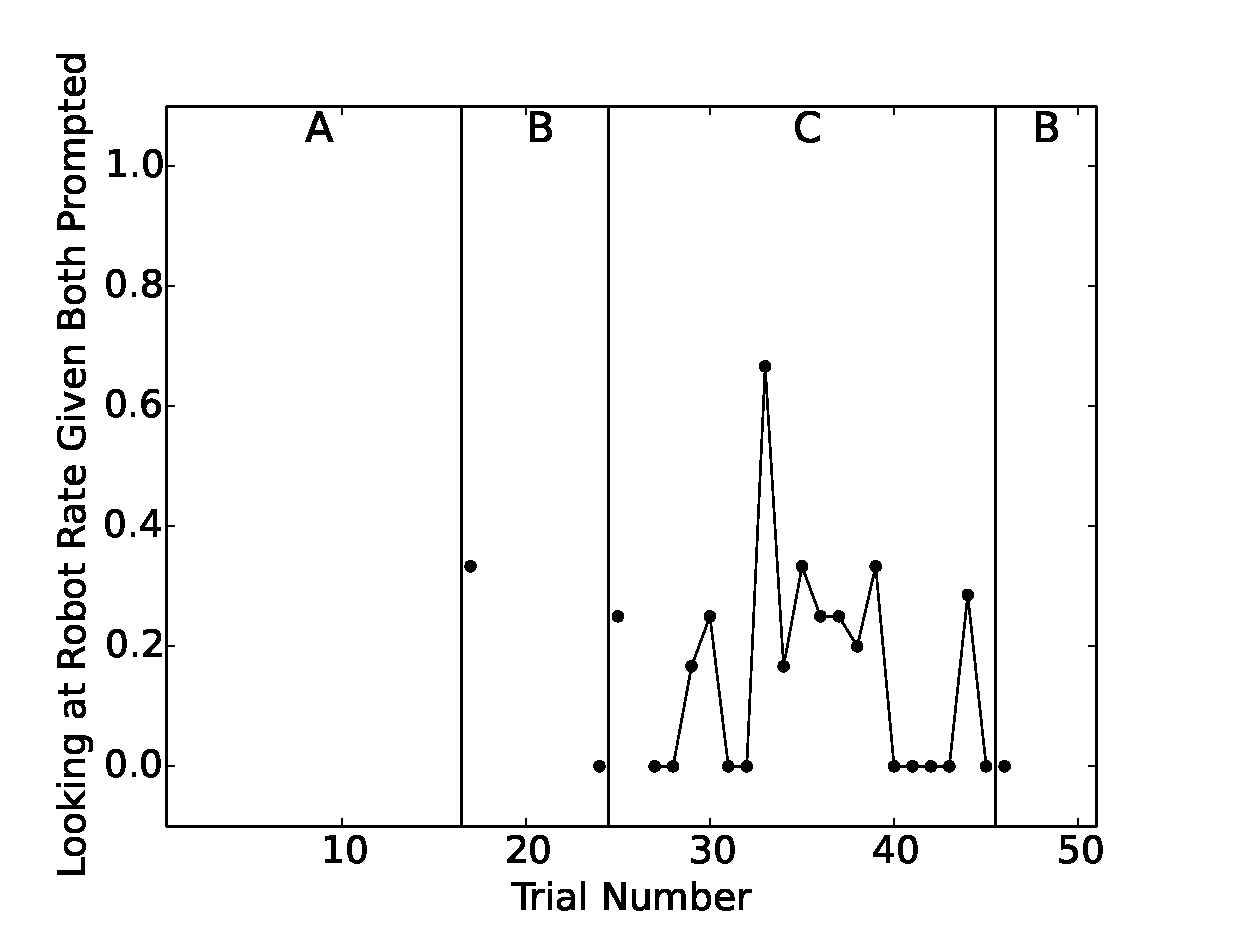
\includegraphics[width=1.1\linewidth]{./img/data_analysis/11LookingatRobotRateGivenBothPrompted.eps}
		\caption{Looking at Robot Rate - Given Both Prompted}
		\label{fig:11LookingatRobotRateGivenBothPrompted}
	\end{subfigure}%
	\caption{Looking at Prompting Agent Rate}
	\label{fig:LookingAtPromptingAgentDuringPrompts}
\end{figure}
